	\section{Data and Empirical Results}
	
	The study is based on a	broad intradaily financial dataset comprising 41 assets listed on the B3 from 2009 to 2017
	
	Our empirical application uses B3's stock returns
	
	In our empirical analysis we have used high frequency data on transaction prices for assets listed on the B3. The sample period ran from December 18, 2009 to February 17, 2017, delivering 1761 distinct days. We have used functions from the “GetHFData” R package by Perlin and Ramos (2016) in different stages of the data cleaning process. In the first step, we discarded any record with a timestamp outside the regular marketing opening hours. Throughout our sample, the official B3 trading day have changed ten times, being the opening time at 10 a.m. or at 11 a.m. and the closing time between 16:55 and 17:55. On holy Wednesday the stock exchange operates half day. Those days were discarded in order to avoid outliers. The same was done on dates in which there were
	delays due to technical failure or matches of the Brazil national team in the 2014 FIFA World Cup, resulting in the elimination of 13 observations. Canceled trades were also deleted. The ticker symbols, names and sector for each of the assets are provided in the appendix (table A.1).
	We adjusted our historical price data to remove gaps caused by stock splits and reverse stock splits in order to prevent misleading signals. Other adjustments were made to remove smaller	gaps caused by different types of corporate actions, such as dividends, bonus issues of shares, rights issues of shares, interest on equity and spinoffs. Such adjustments ensure that all the resulting price movements are caused solely by market forces.
	
	The daily closing price was used to compute squared close to close log returns. They were not part of our intradaily data series, since they are defined by
	an auction, after the regular trading hours.
	
	Beyond this	reason, our choice of sampling frequency is related to the liquidity level of the shares listed in B3.
	
%	B3. (n.d.). Listed Companies. Available at: http://www.bmfbovespa.com.br/en_us/products/listedequities-
%	and-derivatives/equities/listed-companies.htm. Accessed: 2017-06-01.
	
	Our data set consists of daily data of adjusted closing prices of all stocks that belongs to the S\&P 500 market index from July 1990 to December 2015, a time period that covers several market upturns and downturns, as well as relatively calm and volatile periods. We obtain adjusted closing prices from Bloomberg, whereas returns on the Fama and French factors are obtained from French's website\footnote{\url{http://mba.tuck.dartmouth.edu/pages/faculty/ken.french/Data_Library/det_st_rev_factor_daily.html}}. The data set spans 6,426 days and includes a total of 1100 stocks over all periods. Only stocks that are listed during the formation period are included in the analysis, \emph{i.e.}, around 500 stocks in each trading period. We assume that all trades occur at the closing price of that day.
	
	
	Using data from the Center for Research in Security Prices (CRSP) from 1980 to 2006, \citet*{french2008} estimates that the cost of active investing, including total commissions, bid-ask spreads, and other cost investors pay for trading services, has dropped from 146 basis points in 1980 to 11 basis points in 2006. Considering the US stock live trades on the Nyse-Amex between August 1998 and September 2013 for a large institucional investor, \citet*{fim15} estimate that the average trading costs for market impact (MI) and implementation shortfall methodology (IS) are 8.81 and 9.13 basis points, respectively, while the median trading costs are 6.24 and 7.63 basis points, respectively. \citet{avellaneda2010, stubinger2016,liu2017,stubinger2018} assume transaction costs of 5 basis points per share half-turn, thus 10 basis points for the round-trip transaction cost. Following these studies, we assume trading costs of 0.10\% (10 basis points) and 0.20\% (20 basis points) per round-trip pair trade.
	

	
	\vspace{0.3cm}
	
	
	\subsection{Profitability of the Strategies}
	
First, we provide multiple boxplots in Figures \ref{fig:Figure1} and \ref{fig:Figure2} to analyze the sensitivity of the annualized excess returns (Figure \ref{fig:Figure1}) and annualized Sharpe ratios (Figure \ref{fig:Figure2}) when the opening thresholds $\Delta_{1}$ and $\Delta_{2}$ are changed to top 5, 10, 15, 20, 25, 30 and 35 pairs for each of the strategies from 1991/2-2015 on commited capital and on fully invested capital after costs (10 bps)\footnote{The numerical experiments show that the relative performances out-of-sample stay very similar when we consider 20 bps. Since the results are very much alike they are not presented here and are available under request. Hereafter, we consider 10 basis points as transaction costs to report results for the remainder of this paper.}. Pairs are formed based on the smallest sum of squared deviations. The last boxplot (from left to right) shows the performance for the distance strategy (2.0$\sigma$), while the others report the outcomes using multiple opening trigger points for the cumulative mispricing indexes $M_{1,t}$ and $M_{2,t}$ (one above 0.05, 0.1, 0.15, 0.2, 0.25, 0.3, 0.35, 0.4, and 0.55 and the other one below their negative counterparts). Based on these outcomes we perform the subsequent analyses considering 0.2 and -0.2 as the opening thresholds for the mixed copula strategy.

\begin{figure}[!ht]
	\centering
	%\includegraphics[scale=0.26]{fig26.pdf}
	%\includegraphics[width=\linewidth,height=7.5cm]{fig26.pdf}
	%		\resizebox{\linewidth}{!}{\input{Figure1.tex}}
	%		\captionsetup{justification=raggedright,
	%		singlelinecheck=false
	%	}
	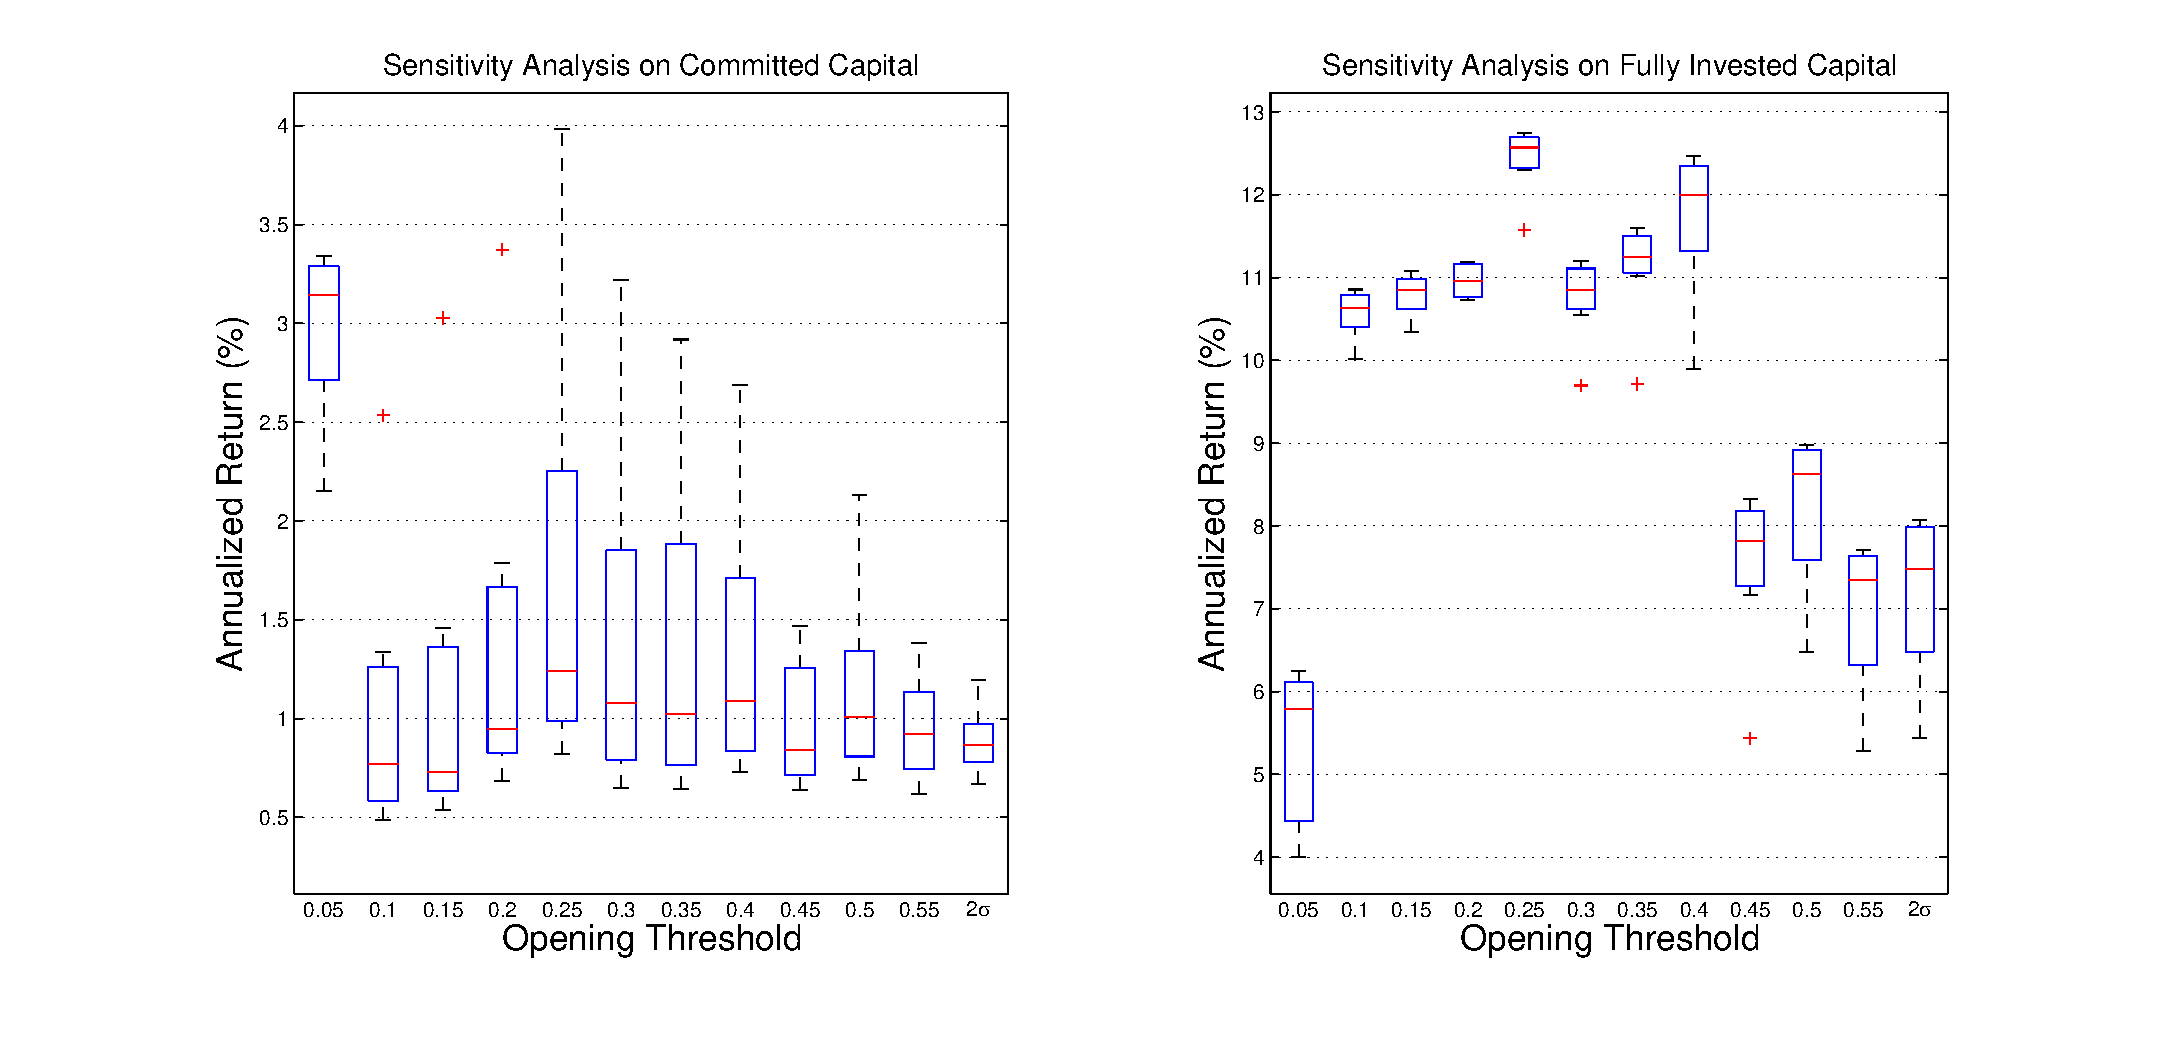
\includegraphics[width=\linewidth]{Figure1.eps}
	\captionsetup{justification=raggedright,
		singlelinecheck=false
	}
	\caption{\textbf{Annualized returns of pairs trading strategies after costs on committed and fully invested capital}}
	\caption*{\scriptsize These boxplots show annualized returns on committed (left) and fully invested (right) capital after transaction cost to different opening thresholds from July 1991 to December 2015 for Top 5 to Top 35 pairs. Pairs are formed based on the smallest sum of squared deviations.}
	\label{fig:Figure1}
\end{figure}

\begin{figure}[!ht]
	\centering
%	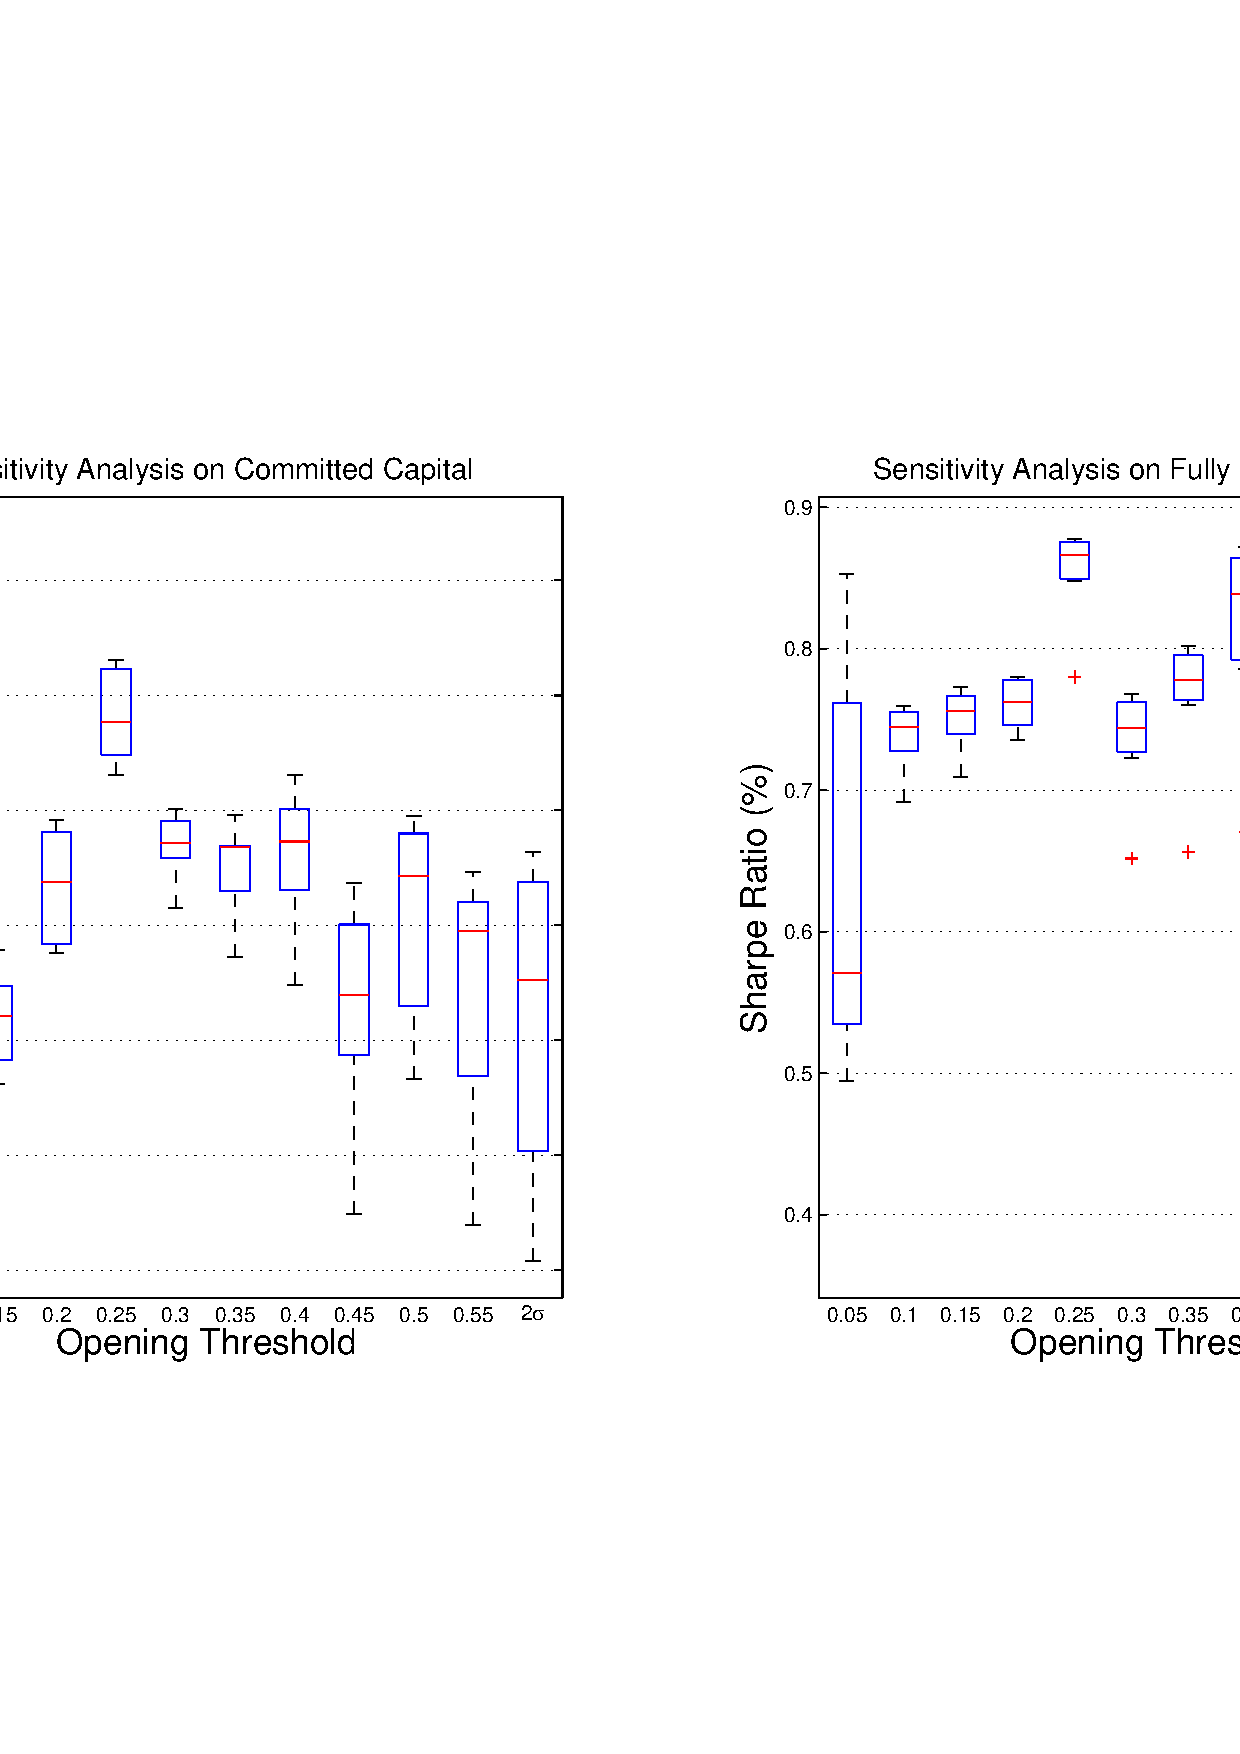
\includegraphics[width=\linewidth,height=7.5cm]{Figure2.pdf}
%	\resizebox{\linewidth}{!}{\input{Figure2.tex}}
%	\captionsetup{justification=raggedright,
%		singlelinecheck=false
%	}
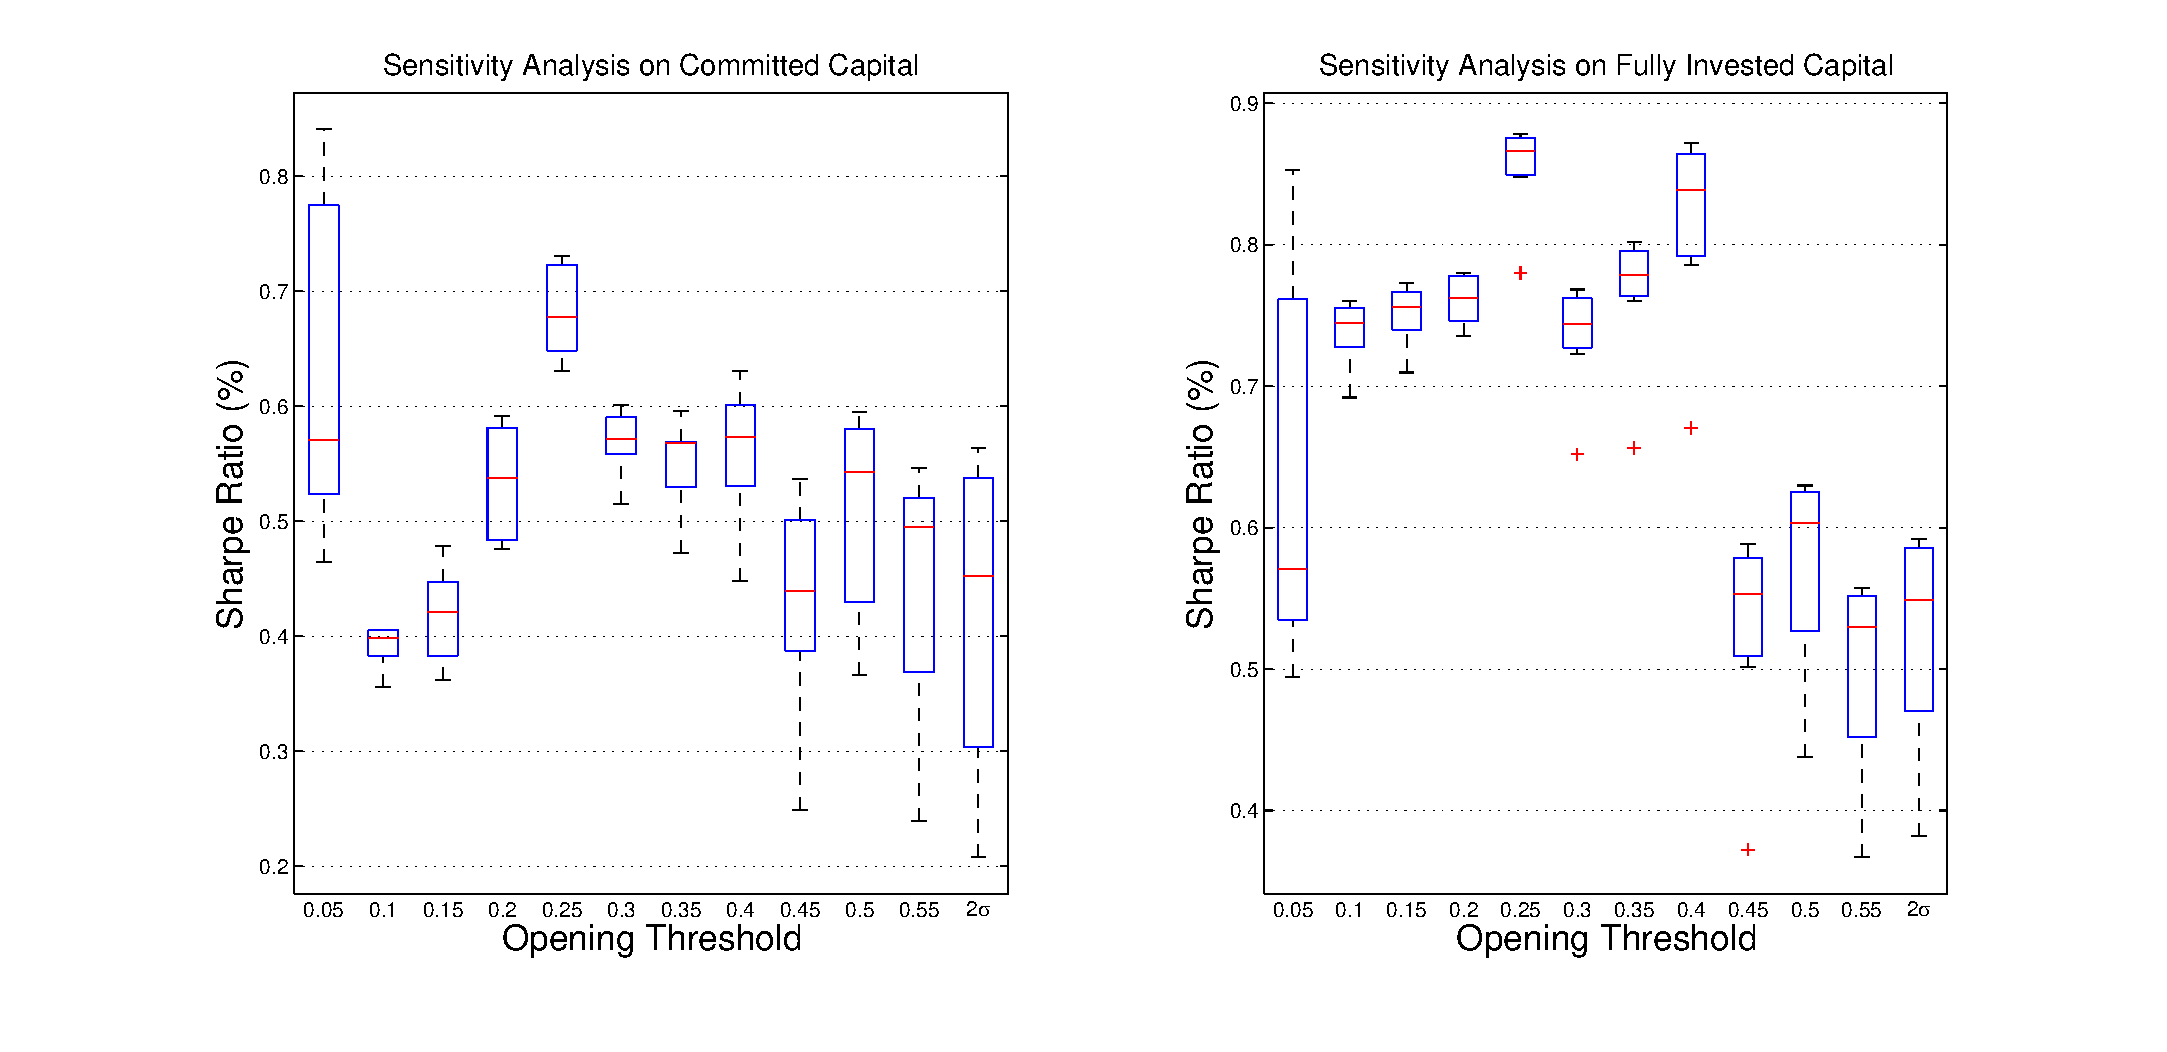
\includegraphics[width=\linewidth]{Figure2.eps}
\captionsetup{justification=raggedright,
	singlelinecheck=false
}
\caption{\textbf {Sharpe ratio of pairs trading strategies after costs on committed and fully invested capital}}
\begin{quote} {\scriptsize These boxplots show Sharpe ratios on committed (left) and fully invested (right) capital after transaction cost to different opening thresholds from July 1991 to December 2015 for Top 5 to Top 35 pairs. Pairs are formed based on the smallest sum of squared deviations.}\end{quote}
\label{fig:Figure2}
\end{figure}

Table \ref{tab:table101} reports annualized mean excess returns, annualized Sharpe and Sortino ratios, \citet*{nw87} adjusted t-statistics, share of negative observations, the maximum drawdown in terms of maximum percentage drop between two consecutive days (MDD1) and between two days within a period of maximum six months (MDD2), annualized standard deviation, minimum and maximum daily return for both strategies from 1991/2-2015, for Top 5 (Panel A), Top 20 (Panel B), and Top 35 (panel C) pairs after costs (10 bps)\footnote{The outcomes are also robust for the other number of pairs considered. Since the results are very much alike they are not presented here and are available under request.}. Furthermore, Section 1 shows the return on Committed Capital and Section 2 on Fully Invested Capital. %Panel A lists the results after transaction costs and Panel B before transaction costs. 	
	
By analyzing Table \ref{tab:table101}, it is possible to observe a series of important facts. First, note that the copula-based pairs strategy outperforms the distance method for Top 5 pairs and committed capital. The mixed copula strategy yields the highest average excess returns (3.98\%), the lowest annualized standard deviation (6.31\%) and reaches a Sharpe ratio of 0.63 after costs, over twice as much as what we get from investing in the tradicional distance method. The Sortino ratio confirms that the mixed copula model offers better risk-adjusted returns. The statistics also indicate that the mixed copula model delivers the highest t-statistics (statistically significant at 1\% and economically large as well) and a lower probability of a negative trade, where the share of days with negative returns (41.79\%) is consistently smaller than the market performance (47.45\% of negative returns over the period). Furthermore, the summary statistics also show that mixed copula method offers better hedges against losses than the distance strategy for Top 5 pairs on committed capital when considering the downside risk statistics MDD1 and MDD2. We find that the number of tradeable signals along the competitive strategies is only equiparable in this study for the case of Top 5 pairs. We will explore this point further in the next subsection.

 The listed results for Top 20 and Top 35 pairs on committed capital show that the distance strategy is more profitable than the mixed copula method, although the Sharpe ratios are similar, indicating that returns are alike when we take into account the risks taken. All profits are statistically significant at 1\%. Overall, the copula method is again a less risky strategy regarding the drawdown measures.

\begin{threeparttable}[H]
	\centering \scriptsize
	\caption{Excess returns of pairs trading strategies on portfolios of Top 5, 20 and 35 pairs after costs.}
	\begin{tabularx}{\textwidth}{@{\extracolsep{\fill}}lllllll@{}}
		\toprule
		& \multicolumn{3}{c}{Distance} & \multicolumn{3}{c}{Mixed Copula} \\\cmidrule{2-4} \cmidrule{5-7}
		& Top 5 & Top 20 & Top 35 & Top 5 & Top 20 & Top 35 \\
		\midrule
		& \multicolumn{6}{c}{\textbf{Section 1: Return on Committed Capital}} \\
		& \multicolumn{6}{c}{\textit {Panel A: after transaction costs}} \\
		Annualized Mean Return (\%) & 2.60  & $3.14^{*}$  & $3.12^{***}$  & 3.98  & 1.24  & 0.82 \\
		Sharpe ratio & 0.31  & 0.65  & 0.77  & 0.63  & 0.64  & 0.73 \\
		Sortino Ratio & 0.58  & 1.13  & 1.36  & 1.08  & 1.04  & 1.19 \\
		t-stat & $1.86^{*}$  & $3.31^{***}$  & $3.92^{***}$  & $3.49^{***}$  & $3.52^{***}$  & $3.95^{***}$ \\
		\% of negative trades & 46.98 & 48.06 & 47.97 & 41.79 & 41.33 & 41.31 \\
		MDD1  & 6.73  & 3.88  & 2.70  & 4.36  & 2.07  & 1.18 \\
		MDD2  & 19.62 & 9.69  & 7.52  & 9.29  & 3.43  & 1.98 \\
		Annualized Std. Dev. (\%) & 8.25  & 4.87  & 4.06  & $6.31^{***}$  & $1.93^{***}$  & $1.12^{***}$ \\
%		Skewness & 0.25  & 0.32  & 0.28  & -0.04 & -0.25 & -0.01 \\
%		Kurtosis & 9.17  & 9.76  & 5.46  & 10.32 & 11.98 & 12.93 \\
		Minimum Daily Return (\%) & -4.43 & -2.76 & -1.50 & -4.16 & -1.47 & -0.84 \\
		Maximum Daily Return (\%) & 5.39  & 2.81  & 1.76  & 3.47  & 0.87  & 0.68 \\
		\midrule
		& \multicolumn{6}{c}{\textit {Panel B: before transaction costs}} \\
		Annualized Mean Return (\%) & 2.90  & $3.43^{**}$  & $3.39^{***}$  & 4.29  & 1.40  & 0.93 \\
		Sharpe ratio & 0.35  & 0.70  & 0.83  & 0.68  & 0.73  & 0.83 \\
		Sortino Ratio & 0.64  & 1.23  & 1.48  & 1.16  & 1.18  & 1.36 \\
		t-stat & $2.04^{**}$  & $3.59^{***}$  & $4.25^{***}$  & $3.73^{***}$  & $3.95^{***}$  & $4.46^{***}$ \\
		\% of negative trades & 46.95 & 47.87 & 47.77 & 41.65 & 41.24 & 41.20 \\
		MDD1  & 6.73  & 3.89  & 2.69  & 4.36  & 2.07  & 1.18 \\
		MDD2  & 19.61 & 9.55  & 7.43  & 9.25  & 3.37  & 1.94 \\
		Annualized Std. Dev. (\%) & 8.27  & 4.88  & 4.07  & $6.33^{***}$  & $1.93^{***}$  & $1.13^{***}$ \\
%		Skewness & 0.26  & 0.33  & 0.29  & -0.04 & -0.23 & 0.07 \\
%		Kurtosis & 9.19  & 9.78  & 5.46  & 10.31 & 11.91 & 12.96 \\
		Minimum Daily Return (\%) & -4.43 & -2.77 & -1.50 & -4.16 & -1.47 & -0.84 \\
		Maximum Daily Return (\%) & 5.41  & 2.81  & 1.77  & 3.47  & 0.87  & 0.68 \\
		\midrule
& \multicolumn{6}{c}{\textbf{Section 2: Return on Fully Invested Capital}} \\
& \multicolumn{6}{c}{\textit {Panel A: after transaction costs}} \\
		Annualized Mean Return (\%) & 4.01  & 6.07  & 5.76  & $11.58^{*}$ & $12.30^{**}$ & $12.73^{**}$ \\
		Sharpe ratio & 0.28  & 0.66  & 0.76  & $0.78^{**}$  & 0.85  & 0.88 \\
		Sortino Ratio & 0.57  & 1.19  & 1.38  & 1.43  & 1.54  & 1.59 \\
		t-stat & $1.81^{*}$  & $3.55^{***}$  & $4.05^{***}$  & $4.26^{***}$  & $4.60^{***}$  & $4.73^{***}$ \\
		\% of negative trades & 46.98 & 48.06 & 47.97 & 41.79 & 41.31 & 41.28 \\
		MDD1  & 8.70  & 5.43  & 4.24  & 9.00  & 9.00  & 9.00 \\
		MDD2  & 38.36 & 20.03 & 15.07 & 25.68 & 25.68 & 25.68 \\
		Annualized Std. Dev. (\%) & 14.51 & $9.20^{***}$  & $7.57^{***}$  & 14.84 & 14.51 & 14.51 \\
%		Skewness & 0.26  & 0.04  & 0.19  & 0.15  & 0.14  & 0.15 \\
%		Kurtosis & 11.27 & 5.85  & 4.04  & 11.07 & 12.28 & 12.35 \\
		Minimum Daily Return (\%) & -8.34 & -4.71 & -3.10 & -10.19 & -10.19 & -10.19 \\
		Maximum Daily Return (\%) & 10.07 & 3.74  & 3.17  & 10.16 & 10.16 & 10.16 \\
		\midrule
& \multicolumn{6}{c}{\textit {Panel B: before transaction costs}} \\ 
		Annualized Mean Return (\%) & 4.49  & 6.56  & 6.24  & $12.30^{**}$ & $13.10^{**}$ & $13.53^{**}$ \\
		Sharpe ratio & 0.31  & 0.71  & 0.82  & $0.82^{**}$  & 0.90  & 0.93 \\
		Sortino Ratio & 0.63  & 1.28  & 1.49  & 1.51  & 1.62  & 1.68 \\
		t-stat & $1.98^{**}$  & $3.81^{***}$  & $4.35^{***}$  & $4.48^{***}$  & $4.84^{***}$  & $4.98^{***}$ \\
		\% of negative trades & 46.95 & 47.87 & 47.77 & 41.65 & 41.24 & 41.20 \\
		MDD1  & 8.71  & 5.43  & 4.23  & 9.00  & 9.00  & 9.00 \\
		MDD2  & 38.30 & 19.89 & 14.93 & 25.60 & 25.60 & 25.60 \\
		Annualized Std. Dev. (\%) & 14.56 & $9.23^{***}$  & $7.60^{***}$  & 14.91 & 14.59 & 0.15 \\
%		Skewness & 0.27  & 0.04  & 0.19  & 0.16  & 0.14  & 0.15 \\
%		Kurtosis & 11.25 & 5.86  & 4.04  & 11.03 & 12.22 & 12.29 \\
		Minimum Daily Return (\%) & -8.34 & -4.71 & -3.10 & -10.19 & -10.19 & -10.19 \\
		Maximum Daily Return (\%) & 10.07 & 3.75  & 3.18  & 10.16 & 10.16 & 10.16 \\
		\bottomrule
\end{tabularx}
\begin{tablenotes}
\item \textit{Note:} \scriptsize Summary statistics of the annualized excess returns, standard devations, Sharpe and Sortino ratios on portfolios of top 5, 20 and 35 pairs between July 1991 and December 2015 (6,173 observations). \textcolor{blue} {Pairs are formed based on the smallest sum of squared deviations}. The t-statistics are computed using Newey-West standard errors with a six-lag correction. The columns labeled MDD1 and MDD2 compute the largest drawdown in terms of maximum percentage drop between two consecutive days and between two days within a period of maximum six months, respectively.
\item \footnotesize $^{\ast\ast\ast}$, $^{\ast\ast}$, $^{\ast}$  significant at 1\%, 5\% and 10\% levels, respectively.
%\item \footnotesize The symbol labels (>) and (<) indicate that the null hypothesis represented in (\ref{eq:eq153}) is rejected in favor of the alternative and that the average excess returns, standard deviation, and Sharpe ratio of the mixed copula strategy are found greater (>) or lower (<) than the average excess returns, standard deviation, and the Sharpe ratio of the distance strategy, respectively.
\end{tablenotes}
\label{tab:table101}
\end{threeparttable}


\vspace{0.6cm}

%albeit with higher volatility.
Section 2 of Table \ref{tab:table101} shows results on fully invested capital scheme. We can note that this approach yields a higher Sharpe of 0.78 and Sortino ratio for the copula-based strategy and the excess return of the portfolio averaged 11.58\% a year (almost three times as large as the return of the committed capital approach), with large and significant Newey-West adjusted t-statistic of 4.26 for Top 5 pairs after costs. Apart from being a more volatile strategy, the mixed copula method consistently outperforms the distance strategy for all pairs considered.

Figure \ref{fig:Figure3} shows cumulative excess returns through the full dataset for both strategies for Top 5 (top), Top 20 (center) and Top 35 (bottom) pairs. The left panels display cumulative returns on committed capital, whereas the right panels on fully invested capital. The patterns found in the figure strengthen the mean returns and t-statistics displayed in Table \ref{tab:table101}. It should be noted that the mixed copula strategy shows a superior out-of-sample performance relative to the distance approach after the subprime mortgage crisis, especially after 2010 for Top 5 pairs (when the number of trades is comparable) on committed capital. 

\begin{figure}[!ht]
	\centering
	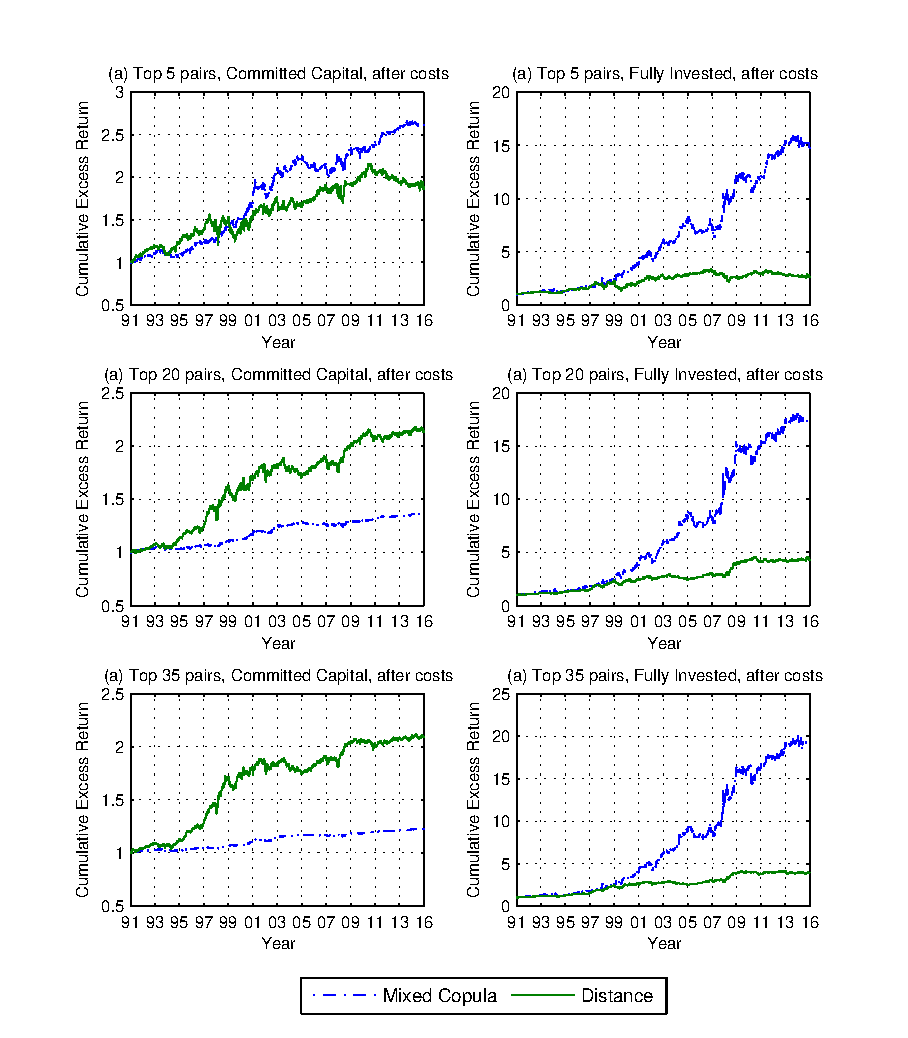
\includegraphics[width=\linewidth]{Figure3.eps}
	\captionsetup{justification=raggedright,
		singlelinecheck=false
	}
	\caption{\textbf{Cumulative excess returns of pairs trading strategies after costs}}
	\caption*{\scriptsize This figure shows how an investment of \$1 evolves from July 1991 to December 2015 for each of the strategies.}
	\label{fig:Figure3}
\end{figure}

Figure \ref{fig:Figure4} shows five-year rolling window Sharpe ratio after costs. The figure reveals mixed results over the long-term period. However, when the number of tradeable signals is similar (Top 5 pairs), the copula-based approach yields the highest five-year Sharpe ratio (up to 1.41) on committed capital in 68.94\% of the days. In 26.22\% of the days over the period the copula method delivers a rolling Sharpe ratio above 1, whereas the distance strategy never attains 1. In fact, the distance approach produces a five-year Sharpe ratio above 0.5 (and most often below zero after 2014) in only 25.4\% of the full period, indicating that the strategy does not reward the risk taken.

For Top 20 and Top 35 pairs on committed capital the strategies show a more competitive pattern. The distance approach presents a greater rolling window Sharpe ratio in 53.37\% and 50.99\% of the days for Top 20 and Top 35 pairs, respectively. However, as we will explore further, the distance approach is a more volatile strategy, identifying a greater number of trading opportunities (more opportunities to make profit) than the copula approach, making the comparison less reliable for a larger number of pairs. The 5-year Sharpe ratios for distance and mixed copula methods are greater than one in 24.97\% and 24.04\% for Top 20 pairs, and 31.92\% and 30.33\% for Top 35 pairs, respectively.

For fully invested weighting scheme the mixed copula approach achieves the highest five-year risk-adjusted statistic over the long-term period in 88.5\%, 69.14\% and 61.8\% of the data sample for Top 5, Top 20 and Top 35 pairs, respectively.


\begin{figure}[!ht]
\centering
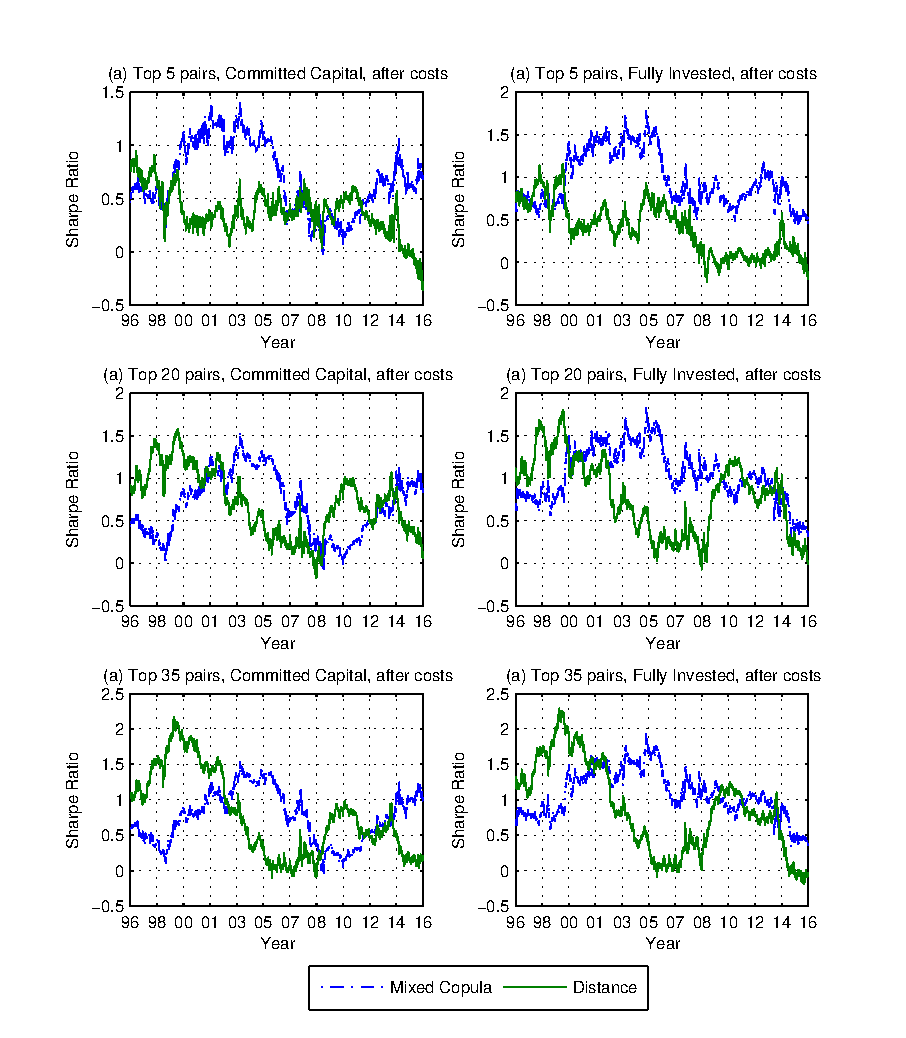
\includegraphics[width=\linewidth]{Figure4.eps}
\captionsetup{justification=raggedright,
	singlelinecheck=false
}
\caption{\textbf{Five-year rolling window Sharpe ratio after costs}}
\caption*{\scriptsize This figure shows how the 5-year rolling window Sharpe ratio evolves from July 1996 to December 2015 for each of the strategies.}
\label{fig:Figure4}
\end{figure}

\vspace{0.6cm}

Figure \ref{fig:Figure5} shows the densities of the five-year Sharpe ratios after costs estimated by means of \citet*{sj1991} bandwidth. As one can see, the densities reinforce our findings in Figure \ref{fig:Figure4}, showing that the right-hand tail of the distribution of the copula-based strategy remains long for Top 5 pairs.


\begin{figure}[!ht]
	\centering
	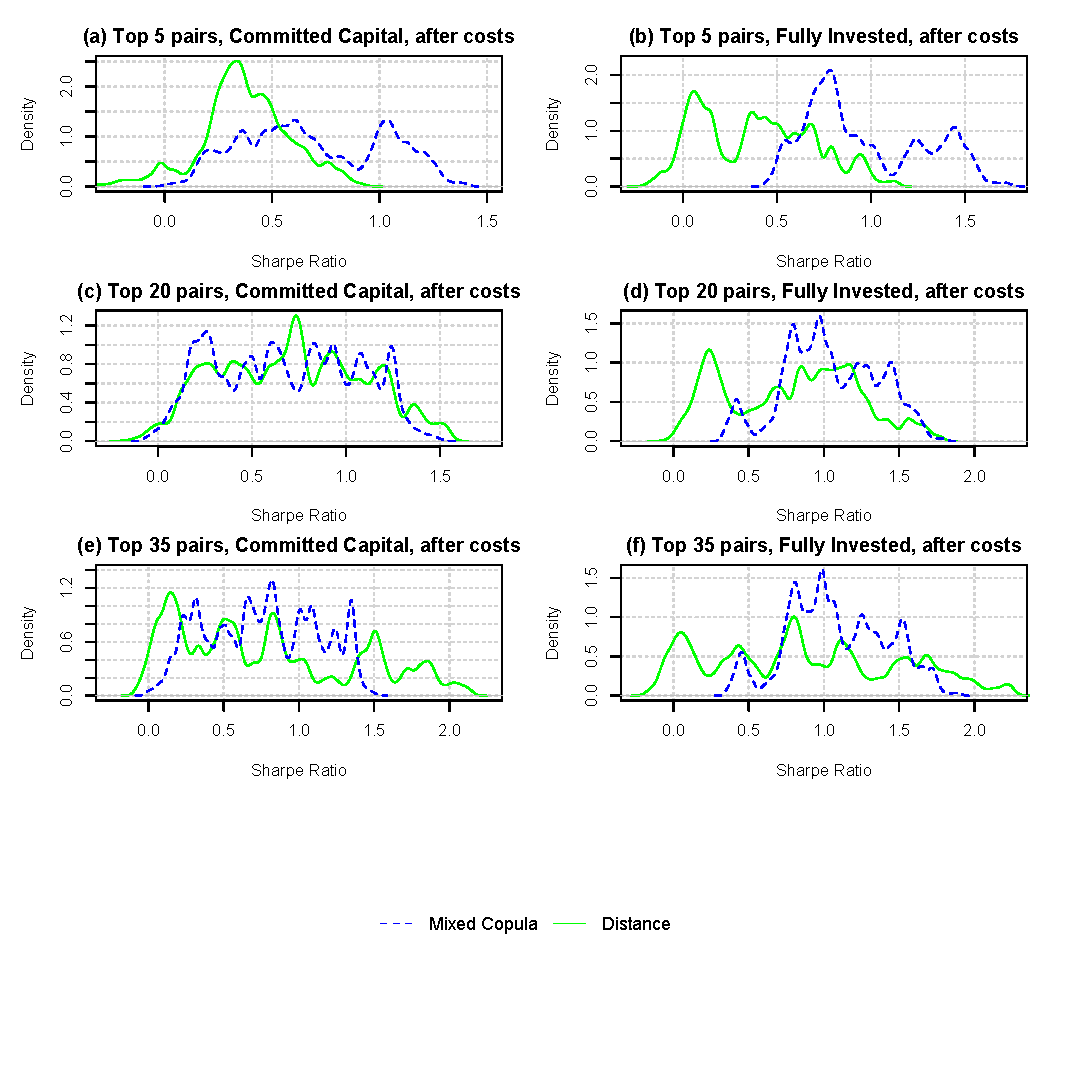
\includegraphics[width=\linewidth]{Figure5.eps}
	\captionsetup{justification=raggedright,
		singlelinecheck=false
	}
	\caption{\textbf{Kernel density estimation of 5-year rolling window Sharpe ratio after costs}}
	\caption*{\scriptsize  This figure shows how the 5-year rolling window Sharpe ratio densities evolve from July 1996 to December 2015 for each of the strategies with \citet*{sj1991}'s bandwidths.}
	\label{fig:Figure5}
\end{figure}

%Robustness checks of the performance of Excess Returns and Sharpe Ratios
One possible criticism might be that the conclusions are based on only one realization of the stochastic process of asset returns computed from the observed series of prices, since among thousands of different strategies is very likely that we find some that show superior performance in terms of excess returns or Sharpe Ratio for this specific realization. In order to mitigate data-snooping criticisms, we use the stationary bootstrap of \citet*{pr94} to compute the bootstrap p-values using the methodology proposed by \citet*{lw08}. 

%\footnote{It allows for weakly dependent correlation over time.}

%The bootstrap method is used to obtain the distribution of a null hypothesis. Here we want to investigate if the average excess return and the Sharpe Ratio of the Copula methods beat the reference (distance) strategies. To construct the distributions, we bootstrapped the original time series $B=10,000$ times. 
Our bootstrapped null distributions result from Theorem 2 of \citet*{pr94}. We select the optimal block length for the stationary bootstrap following \citet*{pw04}. As the optimal bootstrap block-length is different for each strategy, we average\footnote{We also use the optimal block size for each strategy. We find that the results are robust to the optimal block size, and therefore, we do not report them here.} the block-lengths found to proceed the comparisons between the mixed copula and the distance strategies.

To test the hypotheses that the average excess returns, standard deviations and Sharpe ratios of the copula-based strategy are equal to that of distance method, that is,
\begin{equation}
H_{0}:\mu_{c}=\mu_{d},  \ \
\ \  H_{0}:\sigma_{c}=\sigma_{d},
\ \ \textrm{and} \ \ H_{0}:\frac{\mu_{c}}{\sigma_{c}}=\frac{\mu_{d}}{\sigma_{d}},
\label{eq:eq153}
\end{equation}
we compute, following \citet*{davison1997}, a two-sided $p$-value using $B=10,000$ (stationary) bootstrap re-samples as follows:
\begin{equation}
p_{sboot}=
\begin{cases}
2\frac{\sum_{b=1}^{B}\mathbb{I}\{0< t^{\ast(b)}\}+1}{B+1}, &\text{if} ~~median\left\{ t^{\ast \left( 1\right) },...,t^{\ast \left( B\right)}\right\} > 0, \\
2\frac{\sum_{b=1}^{B}\mathbb{I}\{0\geq t^{\ast(b)}\}+1}{B+1}, &\text{otherwise},
\end{cases}
\label{eq:eq152}
\end{equation}
where $\mathbb{I}$ is the indicator function, $t^{\ast(b)}$ are the values in each block stationary bootstrap replication, and B denotes the number of bootstrap replications.

%Table \ref{tab:table101} report the bootstrap $p$-values for testing the null hypotheses represented by (\ref{eq:eq153}). We compare the copula method with each of the distance approaches (0.75 and 2.0 standard deviations) from 1991/2-2015 for all investment scenarios, \emph{i.e.}, without delay and waiting one-day period for the Top 5, Top 20, and Top 35 pairs, respectively, and before and after costs.

%The symbol labels (>) and (<) in Table \ref{tab:table101} indicate that the respective null hypothesis is rejected in favor of the alternative and that the average excess returns, standard deviation, and the Sharpe Ratio of the mixed copula approach are found greater (>) or lower (<) than their respective counterparts from the distance method.

Overall, these results reinforce the ones previously obtained. As it can be observed, the distance approach is more profitable than the copula method, at least at 10\%, for Top 20 and Top 35 pairs on committed capital. On the other hand, the copula approach significantly outperforms the distance strategy in terms of mean excess returns and in risk-adjusted returns when the number of tradeable signals is comparable (Top 5 pairs) on fully invested weighting structure.


\vspace{1.0cm}


	
	\subsection{Trading statistics}
	
	Table \ref{tab:table102} reports trading statistics. Panel A, B and C report results for Top 5, Top 20 and Top 35 pairs, respectively. The average price deviation trigger for opening pairs is listed in the first row of each panel. We can observe that, in average, we initiate the positions before when using the distance approach. The positions are initiated when prices have diverged by 5.94\%, 6.81\%, and 7.29\% for Top 5, Top 20, and Top 35 pairs, respectively. Similar to \citet*{ggr06}, the trigger spread increases with the number of pairs for all approaches\footnote{\citet*{ggr06} explains that the standard deviation of the prices increases as the proximity of the securities in price space decreases, thus increasing the trigger spreads.}.
	
	The table reveals that the average number of pairs traded per six-month period is only equiparable among the strategies for Top 5 pairs. For Top 20 and Top 35 pairs the total number of pairs opened is about 75\% and 138\% greater when starting positions based on the distance approach. This suggests that a two standard deviation trigger as opening criterion \citep{ggr06} is less conservative than the opening threshold suggested by \citet*{rf15} using the cumulative mispricing indexes $M_{1,t}$ and $M_{2,t}$. Thus, the distance approach will be able to identify more trading opportunities to profit making the comparison less meaningful, although in practice the benefits are partly offset by the trading costs.
	
	Finally, note that each pair is held open, in average, by 50.7 and 37.7 trading days (2.4 and 1.8 months) under the distance and copula approaches, respectively, for Top 5 pairs, which indicates that they are a medium-term investment under these strategies.
	
	\begin{threeparttable}[H]
		\centering \scriptsize
		\caption{Trading statistics.}
		\begin{tabularx}{\textwidth}{@{\extracolsep{\fill}}p{7cm}p{1cm}p{1cm}p{1cm}p{1cm}@{}}
			\toprule
			\multicolumn{1}{c}{Strategy} & Distance & Mixed Copula \\
			\midrule
			& \multicolumn{2}{c}{\textit{Panel A: Top 5}} \\
			& &  \\
			Average price deviation trigger for opening pairs & 0.0594 & 0.0665  \\
			Total number of pairs opened &  352   &  348   \\
			Average number of pairs traded per six-month period & 7.18 & 7.10    \\
			Average number of round-trip trades per pair & 1.44 & 1.42   \\
			~~Standard Deviation & 1.0128 & 1.33   \\
			Average time pairs are open in days &  50.70 &  37.70  \\
			~~Standard Deviation & 39.24 & 38.93    \\
			Median time pairs are open in days &  38.5  &  19          \\
			& &  \\
			& \multicolumn{2}{c}{\textit{Panel B: Top20}} \\
			& & \\
			Average price deviation trigger for opening pairs & 0.0681 & 0.0821    \\
			Total number of pairs opened &  1312  &  749     \\
			Average number of pairs traded per six-month period & 26.78 & 15.29   \\
			Average number of round-trip trades per pair & 1.34 & 0.76  \\
			~Standard Deviation & 0.99 & 0.99    \\
			Average time pairs are open in days & 51.65 & 23.60   \\
			~Standard Deviation & 39.62 & 32.90    \\
			Median time pairs are open in days & 41    & 9           \\
			& & \\
			& \multicolumn{2}{c}{\textit{Panel C: Top 35}} \\
			& & \\
			Average price deviation trigger for opening pairs & 0.0729 & 0.0893   \\
			Total number of pairs opened & 2238  & 941   \\
			Average number of pairs traded per six-month period & 45.68 & 19.20 \\
			Average number of round-trip trades per pair & 1.30 & 0.55   \\
			~Standard Deviation & 1.02 & 0.84   \\
			Average time pairs are open in days & 52.72 &  19.35   \\
			~Standard Deviation & 40.48 & 30.56  \\
			Median time pairs are open in days & 42    & 6           \\
	\bottomrule
\end{tabularx}%
\begin{tablenotes}
\item \textit{Note:} \footnotesize  Trading statistics for portfolio of top 5, 20 and 35 pairs between July 1991 and December 2015 (49 periods). \textcolor{blue} {Pairs are formed over a 12-month period according to a minimum-distance (sum of squared deviations) criterion} and then traded over the subsequent 6-month period. Average price deviation trigger for opening a pair is calculated as the price difference divided by the average of the prices.
\end{tablenotes}
\label{tab:table102}%
\end{threeparttable}%
	
	\vspace{1.0cm}
	
	
	
	\subsection{Regression on Fama-French asset pricing factors}
	
	In an attempt to understand the economic drivers behind our data as well as to evaluate whether pairs trading profitability is a compensation for risk, we regress daily excess returns onto various risk factors: daily \citet*{ff15}'s five research factors, the excess return on a broad market portfolio, ($R_{m} - R_{f}$), the difference between the return on a portfolio of small stocks and the return on a portfolio of large stocks ($SMB$, small minus big), the difference between the return on a portfolio of high book-to-market stocks and the return on a portfolio of low book-to-market stocks ($HML$, high minus low), the difference between the return of the most profitable stocks and the return of the least profitable stocks ($RMW$, robust minus weak), the difference between the return of stocks that invest conservatively and the return of stocks that invest aggressively ($CMA$, conservative minus aggressive) plus momentum (Mom),  short-term reversal (SRev), and long-term reversal (LRev) factors, \emph{i.e.},


	\begin{equation}
	\begin{aligned}
	R_{i,t}-R_{f,t}&=\alpha _{i}+\beta _{i}\left( R_{m,t}-R_{f,t}\right)+s_{i}SMB_{t}+h_{i}HML_{t}+r_{i}RMW_{t}\\
	&~+c_{i}CMA_{t}+m_{i}Mom_{t}+v_{i}SRev_{t}+l_{i}LRev_{t}+\varepsilon _{i,t},
	\end{aligned}
	\label{eq:eq101}
	\end{equation}
with $E(\varepsilon _{i,t})=0$, $Var(\varepsilon _{i,t})=\sigma_{\varepsilon _{i}}^{2}$ and $E(\varepsilon _{i,t}\varepsilon _{i,s})=0, t \neq s$, where $i$ and $t$ stands for portfolio and time index, respectively.
	
		All the data used to fit the above regressions are described in and obtained from Kenneth French’s data library\footnote{\url{http://http://mba.tuck.dartmouth.edu/pages/faculty/ken.french/data_library.html}}. We select the model in terms of an approximation to the mean squared prediction error using Bayesian Information Criterion (BIC) \citep{Schwarz1978}. Based on this variable selection procedure we remove the short-term reversal factor from the model. 
	
	The main purpose of these regressions is to estimate the intercept alpha, the average excess return not explained after controlling for these factors, as a measure of risk-adjusted performance. The errors have been adjusted for heteroskedasticity and autocorrelation by using Newey-West adjustment with six lags.
	
	Tables \ref{tab:table103}, \ref{tab:table104} and \ref{tab:table105} report the coefficients and corresponding Newey-West $t$-statistics of regressing monthly portfolio return series onto \citet*{ff15}'s five research factors plus momentum and long-term reversal factors for each of the strategies from 1991/2-2015, after transaction costs, for Top 5, Top 20 and Top 35 pairs, respectively. For each table, Section 1 lists the Return on Committed Capital and Section 2 on Fully Invested Capital. Panel A provides results after transaction costs and Panel B before transaction costs. Tables \ref{tab:table104} and \ref{tab:table105} are provided in Appendix since we want to focus on the case where the number of tradeable signals is comparable. As expected, one could observe that the seven-factor adjusted alphas for Top 20 and Top 35 pairs are in agreement with the patterns found in the center and bottom of Figure \ref{fig:Figure3}.
	
	Table \ref{tab:table103} shows the results for Top 5 pairs. It is clear that the mixed copula approach produces higher adjusted alphas than the distance method for both weighting schemes, especially on fully invested capital (98 basis points with a t-value of 4.17). It should also be noted that the risk-adjusted returns provided by copula and distance strategies are positive and significant at 1\% and 10\%, respectively, after accounting for all the previously mentioned factors. In addition, we find that the alphas of the regressions are significantly positive and higher than the raw excess returns by about 2-7 bps per month, indicating that only a small part of the excess returns can be attributed to their exposures to the seven risk determinants.

	From Table \ref{tab:table103} one could also observe that the magnitude of the loadings on the market factor are larger and with higher t-values for the distance method, and significant at 1\% for both strategies, thus contributing to the pairs trading profitability. Among the other factors, the loadings on the momentum factor are negative and significant at 1\% on committed capital. Furthermore, the portfolios load positively on the HML and load negatively on the SMB and long-term reversal. In addition, the correlation of the excess returns with other traditional equity risk premia factors (RMA and CMW) is nearly zero. Finally, it should be noted that the results show that the exposures to the various sources of systematic profile risk provide a low explanation of the average excess returns for any strategy, with adjusted $R^2$ ranging from  1.4\% to 2.7\%, particularly for the copula-based pairs strategy, indicating that the method is nearly factor-neutral over the whole sample period.
	
%	The SMB coefficients are only significant at 10\% on committed capital for the mixed copula model, whereas the value effect premium (HML factor) slopes are significant at 5\% for the distance approach. In addition, we find that returns are negatively correlated with momentum loadings for both methods at 1\% on committed capital, although a larger negative effect on the performance is found when we use the 2.0 standard deviation threshold. We also find that excess returns are driven by the momentum factor on fully invested capital, although only significant at 5\% for the copula approach. Furthermore, the exposures of pairs trading return strategies to the reversal factor are negative for both weighting schemes and significant at 5\% for the distance approach on committed and fully invested capital, while it is only significant to the less conservative approach for the mixed copula strategy. 
 The regression on asset pricing factors for Top 5 pairs strengthen the patterns found in the Figure \ref{fig:Figure3}, indicating that the mixed copula strategy is able to produce relatively economically larger profits after costs than the distance approach when the number of tradable signals is similar. 

	%\begin{sidewaystable}
	\begin{table}
	\centering \scriptsize
	\caption{Monthly risk profile of Top 5 pairs: \textcolor{blue}{Fama and French} \textcolor{blue}{(2016)}'s five factors plus Momentum and Long-Term Reversal.}\label{tab:table103}%
		\begin{threeparttable}[H]
			\begin{tabularx}{\textwidth}{@{\extracolsep{\fill}} lllllllllll@{}}
				\toprule
				\multicolumn{1}{c}{Strategy} & \multicolumn{1}{c}{Intercept} &  \multicolumn{1}{c}{Rm-Rf} &  \multicolumn{1}{c}{SMB} &  \multicolumn{1}{c}{HML} &  \multicolumn{1}{c}{RMW} &  \multicolumn{1}{c}{CMA} & 
				\multicolumn{1}{c}{Mom} &  \multicolumn{1}{c}{LRev} &  \multicolumn{1}{c}{$R^{2}$} & \multicolumn{1}{c}{$R^{2}_{adj}$} \\
				\midrule
				\multicolumn{11}{c}{\textbf{Section 1: Return on Committed Capital}} \\
				\multicolumn{1}{c}{} & \multicolumn{1}{c}{} & \multicolumn{1}{c}{} & \multicolumn{1}{c}{} & \multicolumn{1}{c}{} & \multicolumn{1}{c}{} & \multicolumn{1}{c}{} & \multicolumn{1}{c}{} & \multicolumn{1}{c}{} & \multicolumn{1}{c}{} & \\
				\multicolumn{1}{c}{Distance} & 0.0025 & 0.0091 & -0.0032 & 0.0113 & 0.0003 & -0.0029 & -0.0107 & -0.0084 & 0.028 & 0.027 \\
				\multicolumn{1}{c}{} & $(1.89)^{*}$ & $(4.22)^{***}$ & (-0.71) & $(2.05)^{**}$ & (0.25) & (-0.18) & $(-4.80)^{***}$ & $(-1.96)^{**}$ & & \\
				\multicolumn{1}{c}{Mixed Copula} &  0.0035 & 0.0052 & -0.0043 & 0.0039 & -0.0035 & 0.0027 & -0.0054 & -0.0057 &  0.015 &  0.014 \\
				\multicolumn{1}{c} {}&  $(3.55)^{***}$ & $(3.68)^{***}$ & $(-1.83)^{*}$ & (1.20) & (-0.99) & (0.63) & $(-2.99)^{***}$ & (-1.57) &  & \\
				
				&       &       &       &       &       &       &       &       &       &       \\
				\midrule
				\multicolumn{11}{c}{\textbf{Section 2: Return on Fully Invested Capital}} \\
				&       &       &       &       &       &       &       &       &       &    \\
				\multicolumn{1}{c}{Distance} & 0.0040 & 0.0170 & -0.0031 & 0.0185 & 0.0049 & -0.0018 & -0.0161 & -0.0150 & 0.025 & 0.024 \\
				\multicolumn{1}{c}{} & $(1.75)^{*}$ & $(4.88)^{***}$ & (-0.45) & $(2.22)^{**}$ & (0.76) & (0.05) & $(-4.30)^{***}$ & $(-1.97)^{**}$ & & \\
				
				\multicolumn{1}{c}{Mixed Copula} &  0.0098 & 0.0148 & -0.0084 & 0.0152 & -0.0053 & 0.0087 & -0.0082 & -0.0222 & 0.018 & 0.017 \\
				\multicolumn{1}{c} {}&  $(4.17)^{***}$ & $(3.51)^{***}$ & -1.45 & 1.6355 & -0.60 & 0.75 & $(-2.19)^{**}$ & $(-2.08)^{**}$ & & \\
				\bottomrule
			\end{tabularx}
			\begin{tablenotes}
				\item \textit{Note:} \footnotesize  This table shows results of regressing monthly portfolio return series onto \textcolor{blue}{Fama and French} \textcolor{blue}{(2016)}'s five factors factors plus momentum and long-term reversal over July 1991 and December 2015 (6173 observations). Section 1 shows the Return on Committed Capital and Section 2 on Fully Invested Capital after transaction costs. Pairs are formed based on the smallest sum of squared deviations. The t-statistics (shown in parentheses) are computed using Newey-West standard errors with six lags.
				\item \footnotesize $^{\ast\ast\ast}$, $^{\ast\ast}$, $^{\ast}$  significant at 1\%, 5\% and 10\% levels, respectively.
			\end{tablenotes}
			\end{threeparttable}%
		\end{table}%
	%\end{sidewaystable}%

\vspace{1.0cm}

\subsection{Sub-period analysis}
The existing literature on trading strategies provides evidence of the sensitivity of performance over different market conditions.  To identify how robust these results are to changes in the market state, we split the full sample period into five sub-periods: (1) July 1991 to December 1995, (2) January 1996 to December 2000, (3) January 2001 to December 2005, (4) January 2006 to December 2010, and (5) January 2011 to December 2015. The third sub-period corresponds to the bear market that comprises the dotcom crisis and the September 11th terrorist attack, whereas the fourth sub-period corresponds to the subprime mortgage financial crisis period.

Figures \ref{fig:Figure6} and \ref{fig:Figure7} show the profitability and risk-adjusted patterns of both strategies for Top 5 (top), Top 20 (center) and Top 35 (bottom) pairs after costs, respectively, for each sub-period on commited capital (left) and fully invested capital (right). 

Overall, the mixed copula strategy yields a superior out-of-sample performance relative to the distance approach in the second and third subperiods (1996-2000 and 2001-2005) and after the subprime mortgage crisis (2011-2015), while the distance method delivers a significant better performance in the first (1991-1995) and fourth subperiods (2006-2010) when the number of trades (Top 5 pairs) are similar on committed capital. Particularly, the distance and mixed copula strategies generated an average annualized excess returns of 3.48\% and 6.84\%, and 3.67\% and 1.56\% over the 2001-2005 and 2006-2010 periods, respectively, which exceeds by far the S\&P 500's average excess returns of -2.28\% and -1.71\% over the same subperiods.

For fully invested weighting scheme the results are consistent with those we have found in the full period analysis (see the right panels in Figure \ref{fig:Figure3}). Specifically, for Top 5 pairs during the main volatile periods, the average excess returns in annual terms was 9.06\% and -0.19\% using the distance approach, and 18.07\% and 9.42\% for the copula-based method.

The results for Top 20 and Top 35 pairs are in agreement with what we expected from previous analyses. The main difference is the performance of the strategies in the second subperiod on committed capital.

\begin{figure}[!ht]
	\centering
		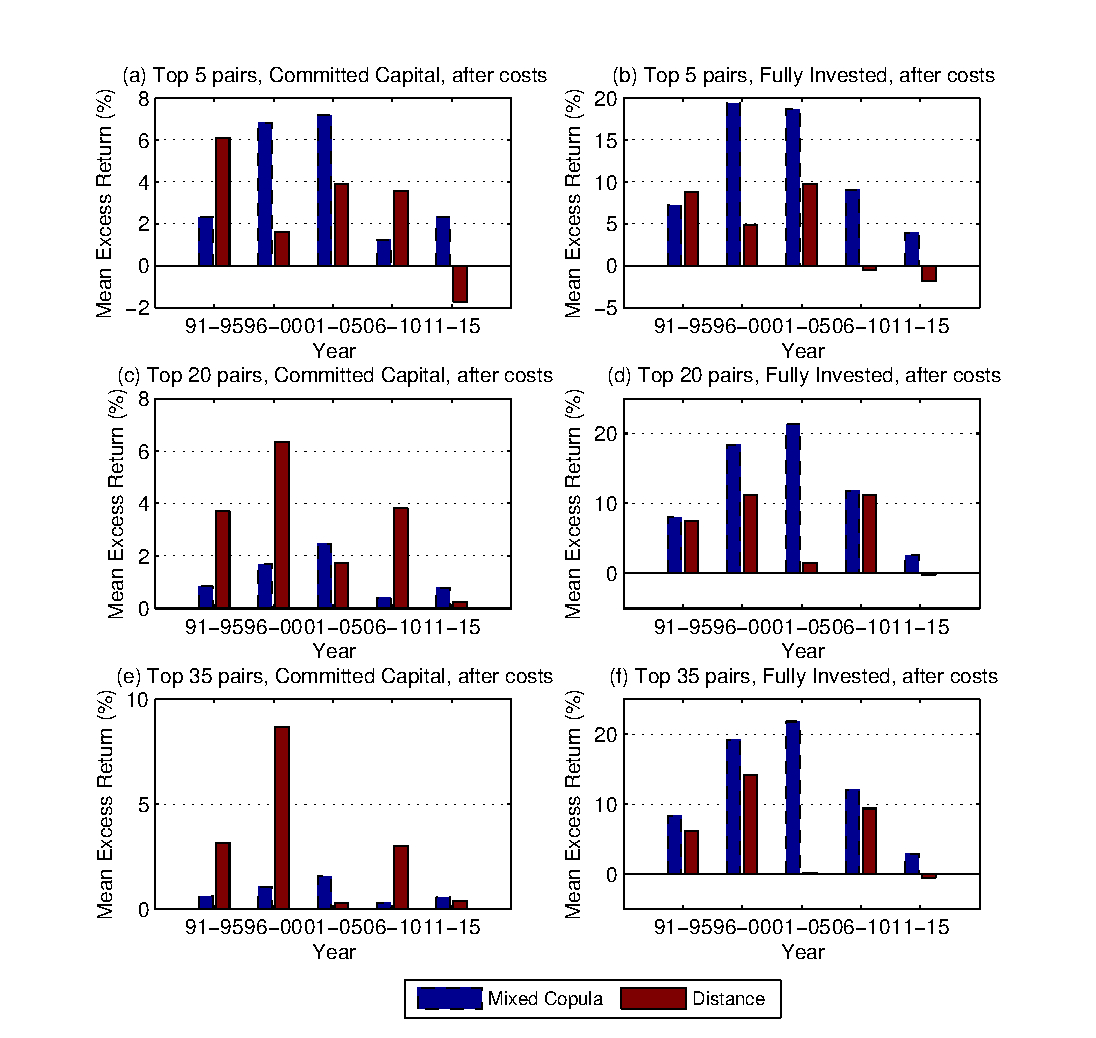
\includegraphics[width=\linewidth]{Figure6.eps}
	\captionsetup{justification=raggedright,
		singlelinecheck=false
	}
	\caption{\textbf{Average excess returns of pairs trading strategies after costs for each sub-period}}
	\caption*{\scriptsize This figure shows how the 5-year rolling window Sharpe ratio densities evolve from July 1996 to December 2015 for each of the strategies.}
	\label{fig:Figure6}
\end{figure}

\begin{figure}[!ht]
	\centering
		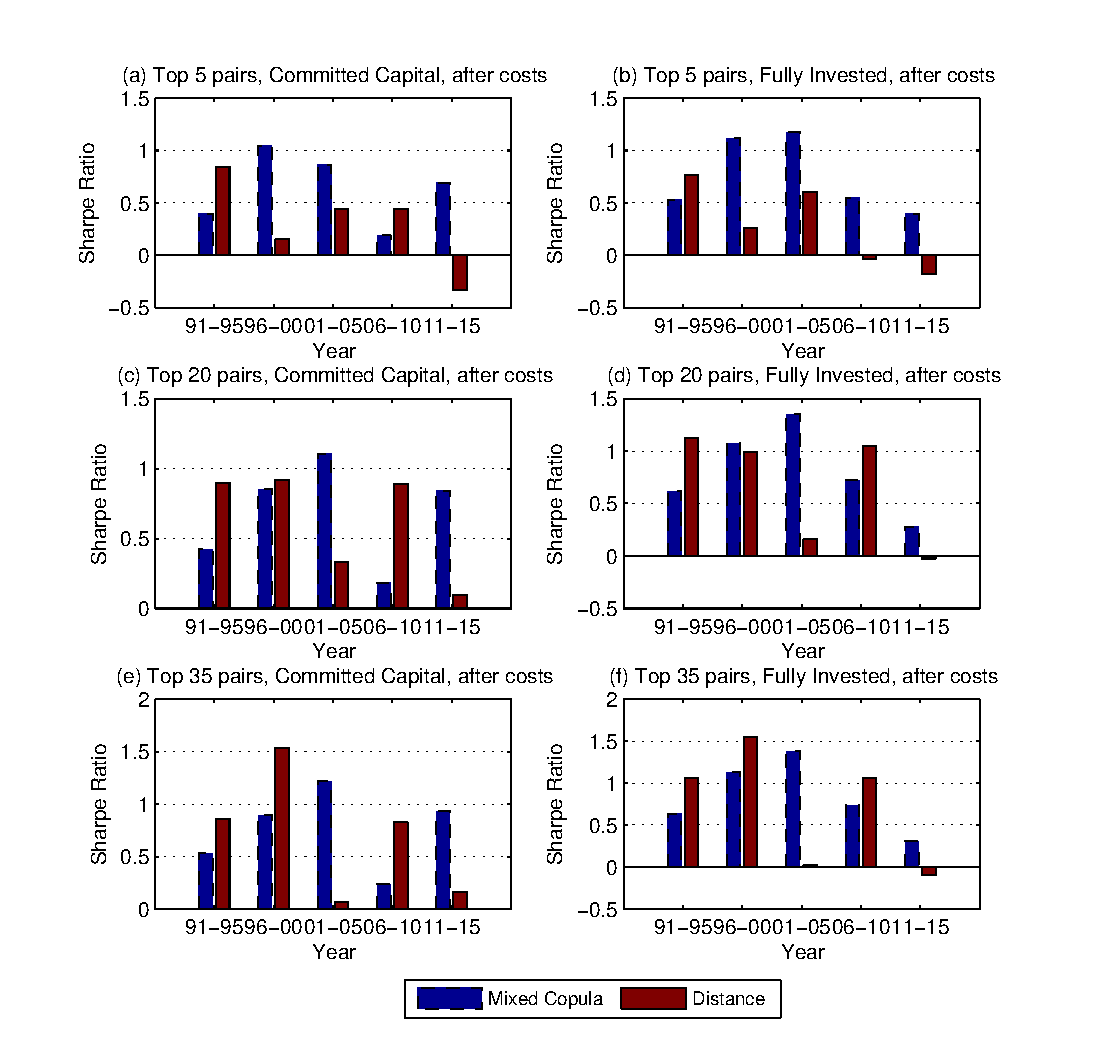
\includegraphics[width=\linewidth]{Figure7.eps}
	\captionsetup{justification=raggedright,
		singlelinecheck=false
	}
	\caption{\textbf{Sharpe Ratio of pairs trading strategies after costs for each sub-period}}
	\caption*{\scriptsize This figure shows how the 5-year rolling window Sharpe ratio densities evolve from July 1996 to December 2015 for each of the strategies.}
	\label{fig:Figure7}
\end{figure}

\vspace{1.0cm}